\section{Methodology}
\label{sec:methodology}
\label{sec:lit-review}
\label{sec:systematization}


\para{Literature Review.}
%
%
To systematize the evolution of web tracking, we perform a literature search (see~\autoref{fig:methodology}) to identify all relevant papers published at any of the following seven venues---IEEE S\&P, USENIX Security, ACM CCS, NDSS, ACM IMC, PETS, and WWW---since their creation (i.e., from 1980 to 2026\footnote{Only papers available on DBLP (\url{https://dblp.org/db/conf}) by June 1st, 2026 were included. Papers were queried using conference-specific paths, e.g., for PETS, we use `conf/pet' (2000-2014) \& `journals/popets' (2015+).}).
%
We obtain a total of 19438 papers that we filter using keywords (see~\refappendix{sec:keywords}) on the title, abstract, or PDF of these publications.
%
These keywords were refined over multiple iterations by discussion among two expert authors.
%
The resulting list of 768 candidate papers is manually reviewed to further exclude  publications unrelated to web tracking techniques, mitigations, or regulatory compliance (e.g., IoT tracking, advertising use cases).



\begin{figure}[!ht]
    \centering
    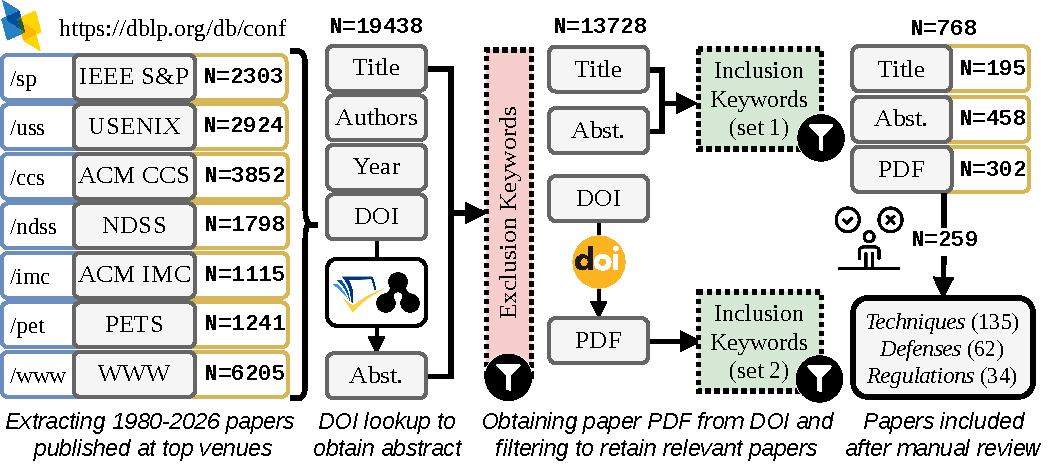
\includegraphics[width=\columnwidth]{figures/methodology.pdf}
    \caption{Overview of our literature search.}% Note that a same paper can be matched along more than one dimension.}
    \label{fig:methodology}
\end{figure}

%%
\begin{table*}[ht]
  \small
\centering
\caption{Summary of systematization criteria and taxonomy for tracking techniques, defenses, and regulatory compliance.}
\label{tab:systematization-criteria}
\renewcommand{\arraystretch}{1}
\begin{tabular}{p{0.004cm} p{7.8cm} p{8.66cm}}
\toprule
& \textbf{Criteria and Description} & \textbf{Taxonomy} \\
\midrule

\multirow[c]{6}{*}{\rotatebox[origin=c]{90}{\textbf{Techniques}}}
 & \textbf{Technique}: What tracking is studied in this research? & See 24 techniques in~\autoref{tab:artifact-capability-matrix}.\\
 & \textbf{Artifact(s)}: What artifact(s) is used by this technique? & See 8 artifact types listed in~\autoref{tab:artifact-taxonomy}. \\
 & \textbf{Capabilities}: What capabilities are required by this technique? & \symInclusion\ Inclusion, \symExecution\ Execution, \symObservation\ Observation, \symStorage\ Storage, \symSharing\ Sharing. \\
 & \textbf{State}: What state does this technique maintain? & Stateful, Stateless, Mixed. \\
 & \textbf{Context}: In what context does it function? & Third-party, First-party, Both. \\
 & \textbf{Goals}: What are the goals of the tracker using this technique? & Same-site, Cross-site, Cross-context. \\
\midrule

\multirow[c]{7}{*}{\rotatebox[origin=c]{90}{\textbf{Defenses}}}
 & \textbf{Technique}: What tracking does this defense protect against? & See 24 techniques in~\autoref{tab:artifact-capability-matrix}.\\
 & \textbf{Artifact(s)}: What artifact(s) does it apply protection to? & See 8 artifact types listed in~\autoref{tab:artifact-taxonomy}. \\
 & \textbf{Development}: Who developed this tracking defense? & Research-based, Industry-based, Community-based. \\
 & \textbf{Deployment}: How is this defense deployed? & \dNative\ In-browser, \dExt\ Extension, \dServer\ Infrastructural, \dTool\ Offline. \\  % server-/network-/protocol-/OS-level
 & \textbf{Support}: What is the support for this defense? & See~\autoref{tab:stateful-tracking-defenses}, \autoref{tab:stateless-tracking-defenses}, and~\autoref{fig:evolution-defenses}. \\
 & \textbf{Goals}: What are the goals of this defense mechanism? & \colorbox{cellred}{Detection \& Blocking} and \colorbox{cellyellow}{Signal Reduction \& Obfuscation}. \\
 & \textbf{Type}: How can the defense mechanism be classified? & See 8 research (\autoref{tab:defense-goal-mechanism-taxonomy}), 23 industry\&community (\autoref{tab:stateful-tracking-defenses}, \autoref{tab:stateless-tracking-defenses}).\\
\midrule

\multirow[c]{3}{*}{\rotatebox[origin=c]{90}{\small\textbf{Policies}}}
& \textbf{Policies}: What regulations and standards are studied? & See EU and US regulations, and standards in ~\autoref{tab:regulations-paper-distribution}. \\
% & \textbf{Policies}: What regulations are studied? & GDPR, CCPA, ePD, CPRA, DSA, DMA, FTC, other (see ~\autoref{fig:evolution-defenses}). \\
% & \textbf{Policies (cont.)}: Which standards and guidelines are studied? & \textit{Standards}: P3P, DNT, GPC. \textit{Guidelines}: CNIL, EDPB, IAB TCF. \\
& \textbf{Aspects}: Which aspects of these policies are covered? & See mapping of 9 policy aspects onto 6 user rights in~\autoref{tab:regulations-aspects}.\\
& \textbf{Compliance}: What are the enforcement challenges?  & Reconciling \colorbox{cellpink}{Incentives}, \colorbox{cellblue}{Expectations}, and \colorbox{cellgreen}{Responsibilities}.\\
% \todo{Abuse, interpretation notices, penalties, trials, precedents.} \todo{gray areas, lack/speed of enforcement}.\\
\midrule
\multirow[c]{2}{*}{\rotatebox[origin=c]{90}{\textbf{Gaps}}}
& \textbf{Open Problems}: What are potential gaps and future directions in the evolution of these techniques, defenses, and regulations? & See the 24 open problems throughout the paper as well as 4 open problems in appendix.\\

\bottomrule
\end{tabular}
% \vspace{-1mm}
\end{table*}

\para{Systematization.}
%
The filtering previously described yields a final set of 255 research papers across the following dimensions: 58 tracking techniques and 108 measurements, 65 defenses, and 34 regulatory compliance papers (see~\refappendix{sec:thematic-analysis} for details).
%
We systematize the evolution of web tracking along these dimensions by following Clarke and Braun’s thematic analysis~\cite{clarke2013successful} that eliminates the need for inter-rater reliability.
%
First, one researcher with expertise in web tracking, reviewed each included paper in detail to evaluate it based on our systematization criteria listed in~\autoref{tab:systematization-criteria}.
%
For each criteria, the expert assigned one or more relevant categories based on the provided description.
%
Next, the evaluator convened with a second expert to deliberate the assigned categories, resolve any ambiguities, and reach a consensus on the final taxonomy to ensure a high quality of analysis as suggested in Clarke and Braun’s approach.
%%
We structure the SoK around this taxonomy and systematize evolution of tracking techniques, defenses, and regulatory compliance, while identifying research gaps and future directions.
%
When needed, we use our domain expertise to complement our explanations with other relevant publications or aspects.



\para{Approach Limitations.}
We acknowledge the following limitations in our approach and our methodology which some are inherent from any SoK effort.
%
\textbf{\textit{Selection Bias.}} We scope our SoK to the seven aforementioned venues where web tracking research has been commonly published, and so, we may have missed other relevant publications.
%
\textbf{\textit{Coding Bias.}} As with any qualitative analysis, our systematization is subject to a degree of subjectivity in how papers are evaluated against the criteria in~\autoref{tab:systematization-criteria}.
We mitigate this following Clarke and Braun's thematic analysis approach~\cite{clarke2013successful} coupled with our domain expertise.
%
While this reduces inconsistencies, it is still possible that other researchers may arrive at slightly varying interpretations of the taxonomy.
%
\textbf{\textit{Focus on EU and US Regulations.}} We scope our approach to the EU and US contexts because they are the closest to our expertise and their regulations have often been precursors to others around the globe\footnote{See \url{https://cnil.fr/en/data-protection-around-the-world}} (LGPD in Brazil, DPDPA in India, Data Protection Act in the U.K., etc.).
For a broader exploration of privacy regulations elsewhere and their nuances, we refer readers to the following SoK from Birrell et al. ~\cite{birrellSoKTechnicalImplementation2024}.
%
\textbf{\textit{Scope coverage.}} We consider adjacent topics such as advertising out-of-scope. Also, we focus on systematizing high-level advances across literature rather than detailing findings from individual papers.